

\title{Lattice based cryptography}
\author{Qaiser khan }
\date{August 2022}


\maketitle

\section{About Me}
 This is Qaiser khan from Pakistan. Pakistan is geographically located in South Asia. I am a PhD student at UCCS, Doing PhD in security and works with Dr Sang Yoon Chang at Network Security and System lab.  I have completed my master’s in information security (with a major in Cryptography) from one of the prestigious universities of Pakistan i.e. National University of Science and Technology, Pakistan. Then I got Research Assistant-ship at UCCS.I like travelling, hiking and love to play with mathematical stuff.I am taking this course CS-6000 because my advisor and my lab mates suggested to take this course and this will help in your research and can learn more new stuff and tools like Zotero, overleaf and also how to use google scholar to find your interest paper more quick.This subject will help to know about good conference, journals and impact factors of journals. My research interest in post quantum cryptography as we know that after Quantum computer came there will be security threat to recent asymmetric algorithm like RSA, Diffie-hellman and all algorithm that is based on factorization and discrete logarithms \cite{alagic2019status}. So to secure the confidential data NIST (National institute of standards and Technology) in 2016 announced for post quantum algorithms that should be quantum resistance\cite{raavi2021security}.

\begin{figure}[htp]
    \centering
    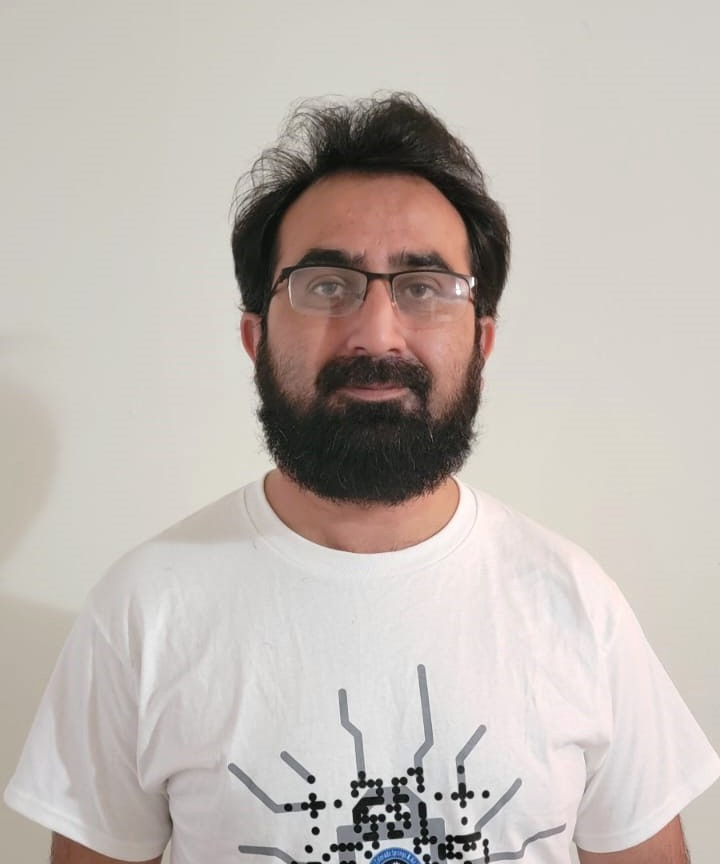
\includegraphics[width=6cm]{qaiser.jpeg}
    \caption{Qaiser khan}
    \label{fig:Qaiser}
\end{figure}

\section{Git Code}
I am working on post-quantum cryptography, so here is the link to a popular library that contains all the NIST standardization source code files for the post-quantum algorithms:
\href{https://github.com/open-quantum-safe/liboqs}{https://github.com/open-quantum-safe/liboqs}.

\section{Any Questions?}


Hi Qaiser, trust you are well.
Your research area seems interesting, does asymmetric algorithm give promise to unbreakable security?...This is Rono
%

% What are the likely methods used to secure asymmetric algorithms?
Do you plan on creating or revising any of the post quantum algorithms? Also, which one do you think shows the most promise/strength? - Dustin Trujillo 

%
%
